% Figure 1: OmicsLake Architecture - Standalone LaTeX Document
% Compile with: pdflatex figure1_architecture_standalone.tex
%
% For embedding in a journal article, copy the tikzpicture environment
% to your main document and add required packages to the preamble.

\documentclass[border=10pt]{standalone}
\usepackage{tikz}
\usetikzlibrary{shapes.geometric, arrows.meta, positioning, fit, backgrounds, calc}
\usepackage[T1]{fontenc}
\usepackage{helvet}
\renewcommand{\familydefault}{\sfdefault}

\begin{document}

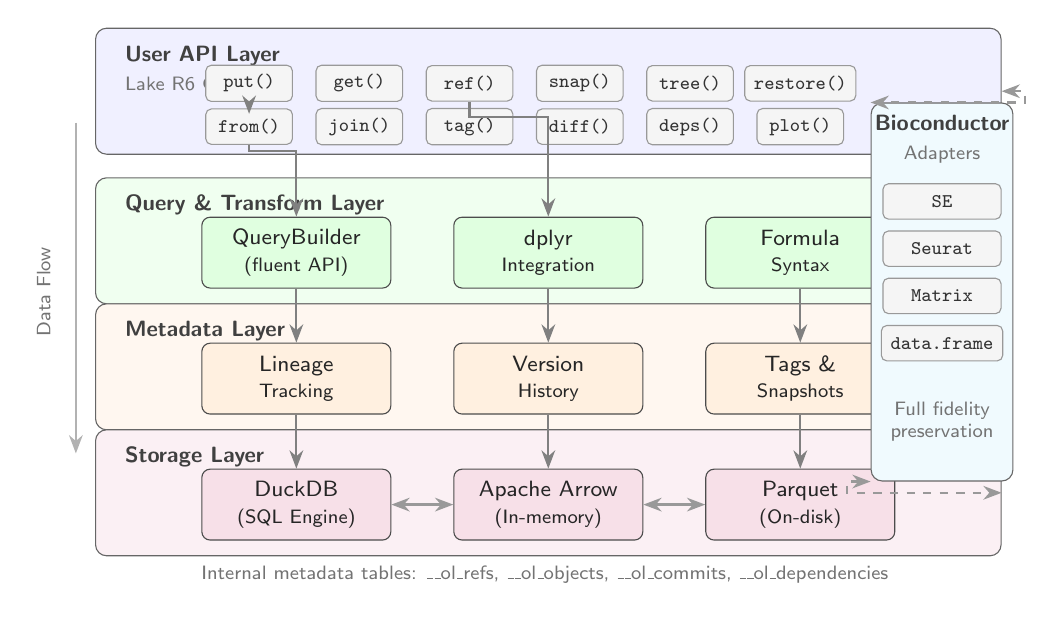
\begin{tikzpicture}[
    % Define styles
    layer/.style={
        draw=black!60,
        fill=white,
        rounded corners=4pt,
        minimum width=11.5cm,
        minimum height=1.6cm
    },
    component/.style={
        draw=black!70,
        fill=#1,
        rounded corners=3pt,
        minimum width=2.4cm,
        minimum height=0.9cm,
        font=\footnotesize,
        align=center,
        text=black!85
    },
    method/.style={
        draw=black!40,
        fill=gray!8,
        rounded corners=2pt,
        minimum width=1.1cm,
        minimum height=0.45cm,
        font=\scriptsize\ttfamily,
        text=black!80
    },
    arrow/.style={
        ->,
        >=Stealth,
        thick,
        black!60
    },
    bidiarrow/.style={
        <->,
        >=Stealth,
        thick,
        black!60
    },
    layerlabel/.style={
        font=\footnotesize\bfseries,
        text=black!75
    },
    sublabel/.style={
        font=\scriptsize,
        text=black!55
    }
]

% ============================================================
% Layer 1: User API (top)
% ============================================================
\node[layer, fill=blue!6] (api_layer) at (0, 5.4) {};
\node[layerlabel, anchor=north west] at (-5.5, 6.1) {User API Layer};
\node[sublabel, anchor=north west] at (-5.5, 5.7) {Lake R6 Class};

% Primary API methods (row 1)
\node[method] (put) at (-3.8, 5.5) {put()};
\node[method] (get) at (-2.4, 5.5) {get()};
\node[method] (ref) at (-1.0, 5.5) {ref()};
\node[method] (snap) at (0.4, 5.5) {snap()};
\node[method] (tree) at (1.8, 5.5) {tree()};
\node[method] (restore) at (3.2, 5.5) {restore()};

% Secondary methods (row 2)
\node[method] (from) at (-3.8, 4.95) {from()};
\node[method] (join) at (-2.4, 4.95) {join()};
\node[method] (tag) at (-1.0, 4.95) {tag()};
\node[method] (diff) at (0.4, 4.95) {diff()};
\node[method] (deps) at (1.8, 4.95) {deps()};
\node[method] (plot) at (3.2, 4.95) {plot()};

% ============================================================
% Layer 2: Query & Transform
% ============================================================
\node[layer, fill=green!6] (query_layer) at (0, 3.5) {};
\node[layerlabel, anchor=north west] at (-5.5, 4.2) {Query \& Transform Layer};

\node[component=green!12] (qb) at (-3.2, 3.35) {QueryBuilder\\{\scriptsize(fluent API)}};
\node[component=green!12] (dplyr) at (0, 3.35) {dplyr\\{\scriptsize Integration}};
\node[component=green!12] (formula) at (3.2, 3.35) {Formula\\{\scriptsize Syntax}};

% ============================================================
% Layer 3: Metadata & Lineage
% ============================================================
\node[layer, fill=orange!6] (meta_layer) at (0, 1.9) {};
\node[layerlabel, anchor=north west] at (-5.5, 2.6) {Metadata Layer};

\node[component=orange!12] (lineage) at (-3.2, 1.75) {Lineage\\{\scriptsize Tracking}};
\node[component=orange!12] (versions) at (0, 1.75) {Version\\{\scriptsize History}};
\node[component=orange!12] (refs) at (3.2, 1.75) {Tags \&\\{\scriptsize Snapshots}};

% ============================================================
% Layer 4: Storage Backend
% ============================================================
\node[layer, fill=purple!6] (storage_layer) at (0, 0.3) {};
\node[layerlabel, anchor=north west] at (-5.5, 1.0) {Storage Layer};

\node[component=purple!12] (duckdb) at (-3.2, 0.15) {DuckDB\\{\scriptsize(SQL Engine)}};
\node[component=purple!12] (arrow) at (0, 0.15) {Apache Arrow\\{\scriptsize(In-memory)}};
\node[component=purple!12] (parquet) at (3.2, 0.15) {Parquet\\{\scriptsize(On-disk)}};

% ============================================================
% Bioconductor Integration (side panel)
% ============================================================
\node[
    draw=black!60,
    fill=cyan!6,
    rounded corners=4pt,
    minimum width=1.8cm,
    minimum height=4.8cm,
    align=center
] (bioc) at (5.0, 2.85) {};

\node[layerlabel] at (5.0, 5.0) {Bioconductor};
\node[sublabel] at (5.0, 4.6) {Adapters};

\node[method, minimum width=1.5cm] (se) at (5.0, 4.0) {SE};
\node[method, minimum width=1.5cm] (seurat) at (5.0, 3.4) {Seurat};
\node[method, minimum width=1.5cm] (matrix) at (5.0, 2.8) {Matrix};
\node[method, minimum width=1.5cm] (df) at (5.0, 2.2) {data.frame};

\node[sublabel, align=center] at (5.0, 1.2) {Full fidelity\\preservation};

% ============================================================
% Layer Connections (vertical flow)
% ============================================================
% API to Query
\draw[arrow, black!50] (put.south) -- ++(0,-0.15);
\draw[arrow, black!50] (ref.south) -- ++(0,-0.2) -| (dplyr.north);
\draw[arrow, black!50] (from.south) -- ++(0,-0.08) -| (qb.north);

% Query to Metadata
\draw[arrow, black!50] (qb.south) -- (lineage.north);
\draw[arrow, black!50] (dplyr.south) -- (versions.north);
\draw[arrow, black!50] (formula.south) -- (refs.north);

% Metadata to Storage
\draw[arrow, black!50] (lineage.south) -- (duckdb.north);
\draw[arrow, black!50] (versions.south) -- (arrow.north);
\draw[arrow, black!50] (refs.south) -- (parquet.north);

% Storage horizontal connections
\draw[bidiarrow, black!40] (duckdb.east) -- (arrow.west);
\draw[bidiarrow, black!40] (arrow.east) -- (parquet.west);

% Bioconductor connections (dashed)
\draw[bidiarrow, dashed, black!40] (api_layer.east) -- ++(0.3,0) |- (bioc.north west);
\draw[bidiarrow, dashed, black!40] (bioc.south west) -| ++(-0.3,0) |- (storage_layer.east);

% ============================================================
% Annotations
% ============================================================
% Data flow indicator
\node[sublabel, rotate=90, anchor=south] at (-6.2, 2.85) {Data Flow};
\draw[arrow, black!30] (-6.0, 5.0) -- (-6.0, 0.8);

% Internal tables
\node[sublabel, anchor=north, align=center] at (0, -0.5) {
    Internal metadata tables: \_\_ol\_refs, \_\_ol\_objects, \_\_ol\_commits, \_\_ol\_dependencies
};

\end{tikzpicture}

\end{document}
